\documentclass[9pt,a4paper]{article}
\usepackage[utf8]{inputenc}
\usepackage[margin=0.55in,top=0.45in,bottom=0.5in]{geometry}
\usepackage{graphicx}
\usepackage{xcolor}
\usepackage{hyperref}
\usepackage{titlesec}
\usepackage{enumitem}
\usepackage{tcolorbox}
\usepackage{booktabs}
\usepackage{caption}
\usepackage{microtype}
\usepackage{multicol}
\usepackage{tabularx}
\usepackage{float}

\definecolor{primary}{HTML}{1A237E}
\definecolor{highlight}{HTML}{7E57C2}
\definecolor{action}{HTML}{F57C00}
\definecolor{lightbg}{HTML}{EDE7F6}

\titleformat{\section}{\normalsize\bfseries\color{primary}}{}{0em}{}[\titlerule]
\titleformat{\subsection}{\small\bfseries\color{highlight}}{}{0em}{}
\titlespacing*{\section}{0pt}{1.2ex plus 0.5ex}{0.5ex plus .2ex}
\titlespacing*{\subsection}{0pt}{0.6ex plus 0.3ex}{0.2ex plus .1ex}

\setlength{\parskip}{0.25em}
\setlength{\parindent}{0em}
\setlength{\abovecaptionskip}{3pt}
\setlength{\belowcaptionskip}{0pt}
\newcommand{\rupee}{INR\,}

\title{\vspace{-2cm}\LARGE \textbf{FinMentor AI \& ArthaScan} \\ \normalsize A Unified Architecture for Zero-Hallucination Financial Advice}
\author{\textbf{Hackathon Submission: PS 9 -- AI Money Mentor}}
\date{\vspace{-1.5em}March 29, 2026}

\begin{document}
\maketitle
\vspace{-1.5em}

% ─── Executive Summary ─────────────────────────────────────────────────────────
\begin{tcolorbox}[colback=blue!4!white,colframe=primary,title={\small Executive Summary},boxsep=2pt,left=4pt,right=4pt,top=2pt,bottom=2pt]
\small The FinMentor AI ecosystem addresses automated financial advice's core problem: \textbf{Trust vs.\ Generative Noise}. Our ``Zero-Hallucination'' architecture isolates all mathematical logic from LLMs. LLMs handle \emph{only} data extraction, voice transcription, and conversational translation --- \textbf{100\% of financial truths} come from deterministic Python engines. Delivered via a \textbf{React Web Dashboard} and \textbf{Telegram Bot}, connected by shared sessions for seamless cross-channel transitions.
\end{tcolorbox}

% ─── Screenshots ───────────────────────────────────────────────────────────────
\begin{figure}[H]
\centering
\setlength{\tabcolsep}{3pt}
\begin{tabular}{cccc}
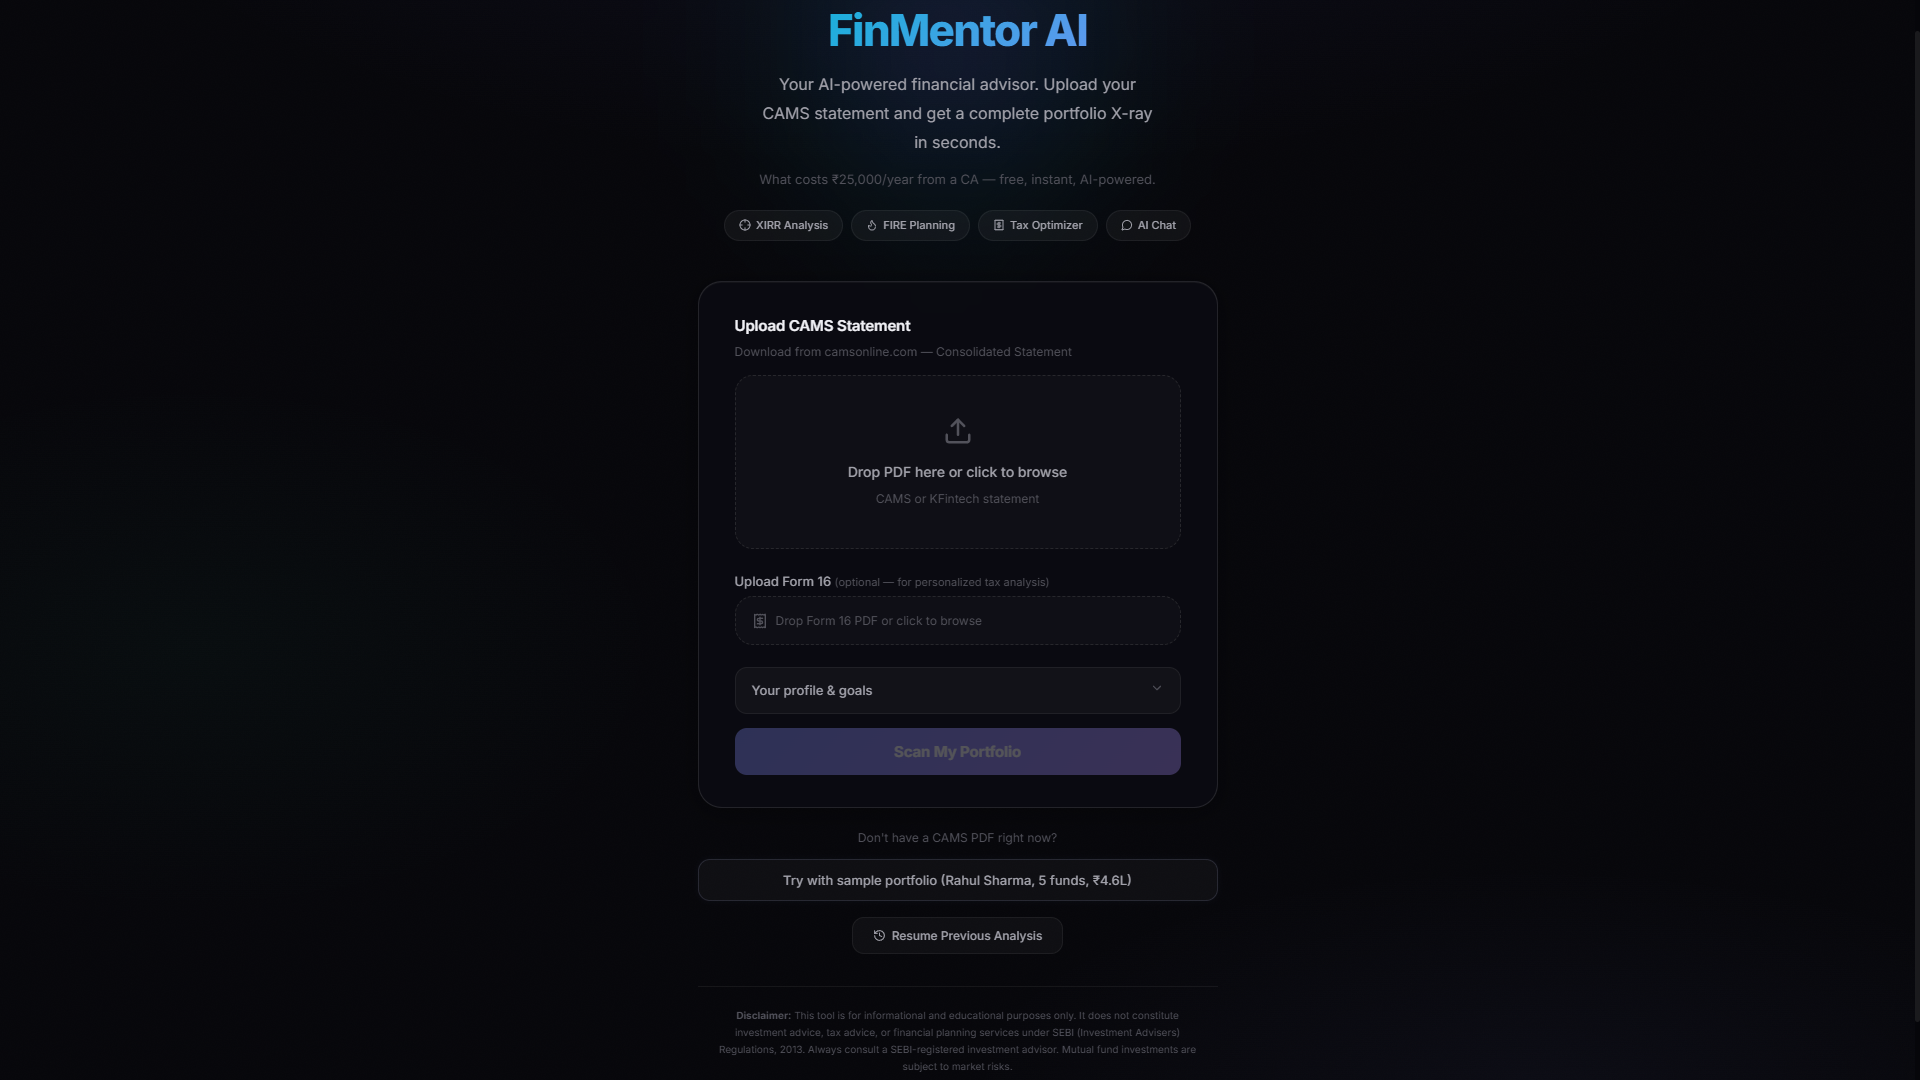
\includegraphics[width=0.23\textwidth]{screenshot_upload.png} &
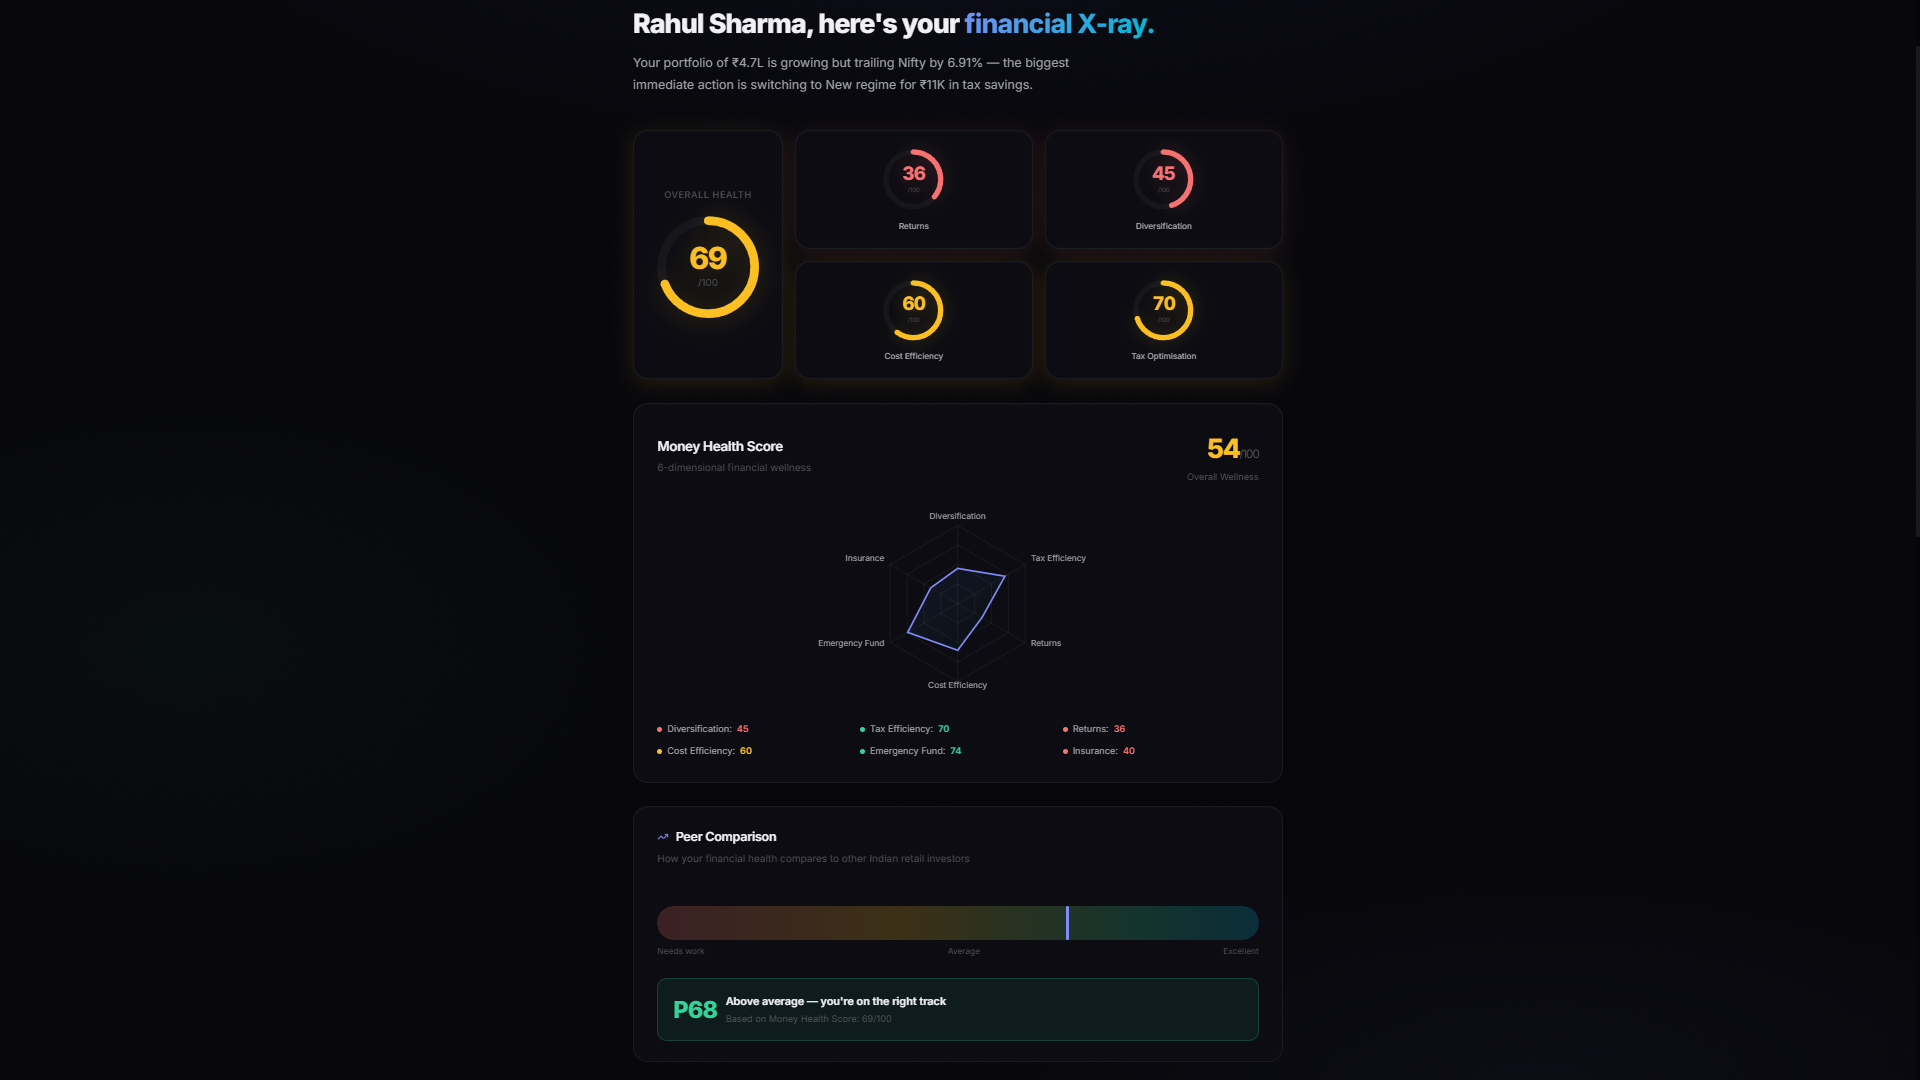
\includegraphics[width=0.23\textwidth]{screenshot_verdict.png} &
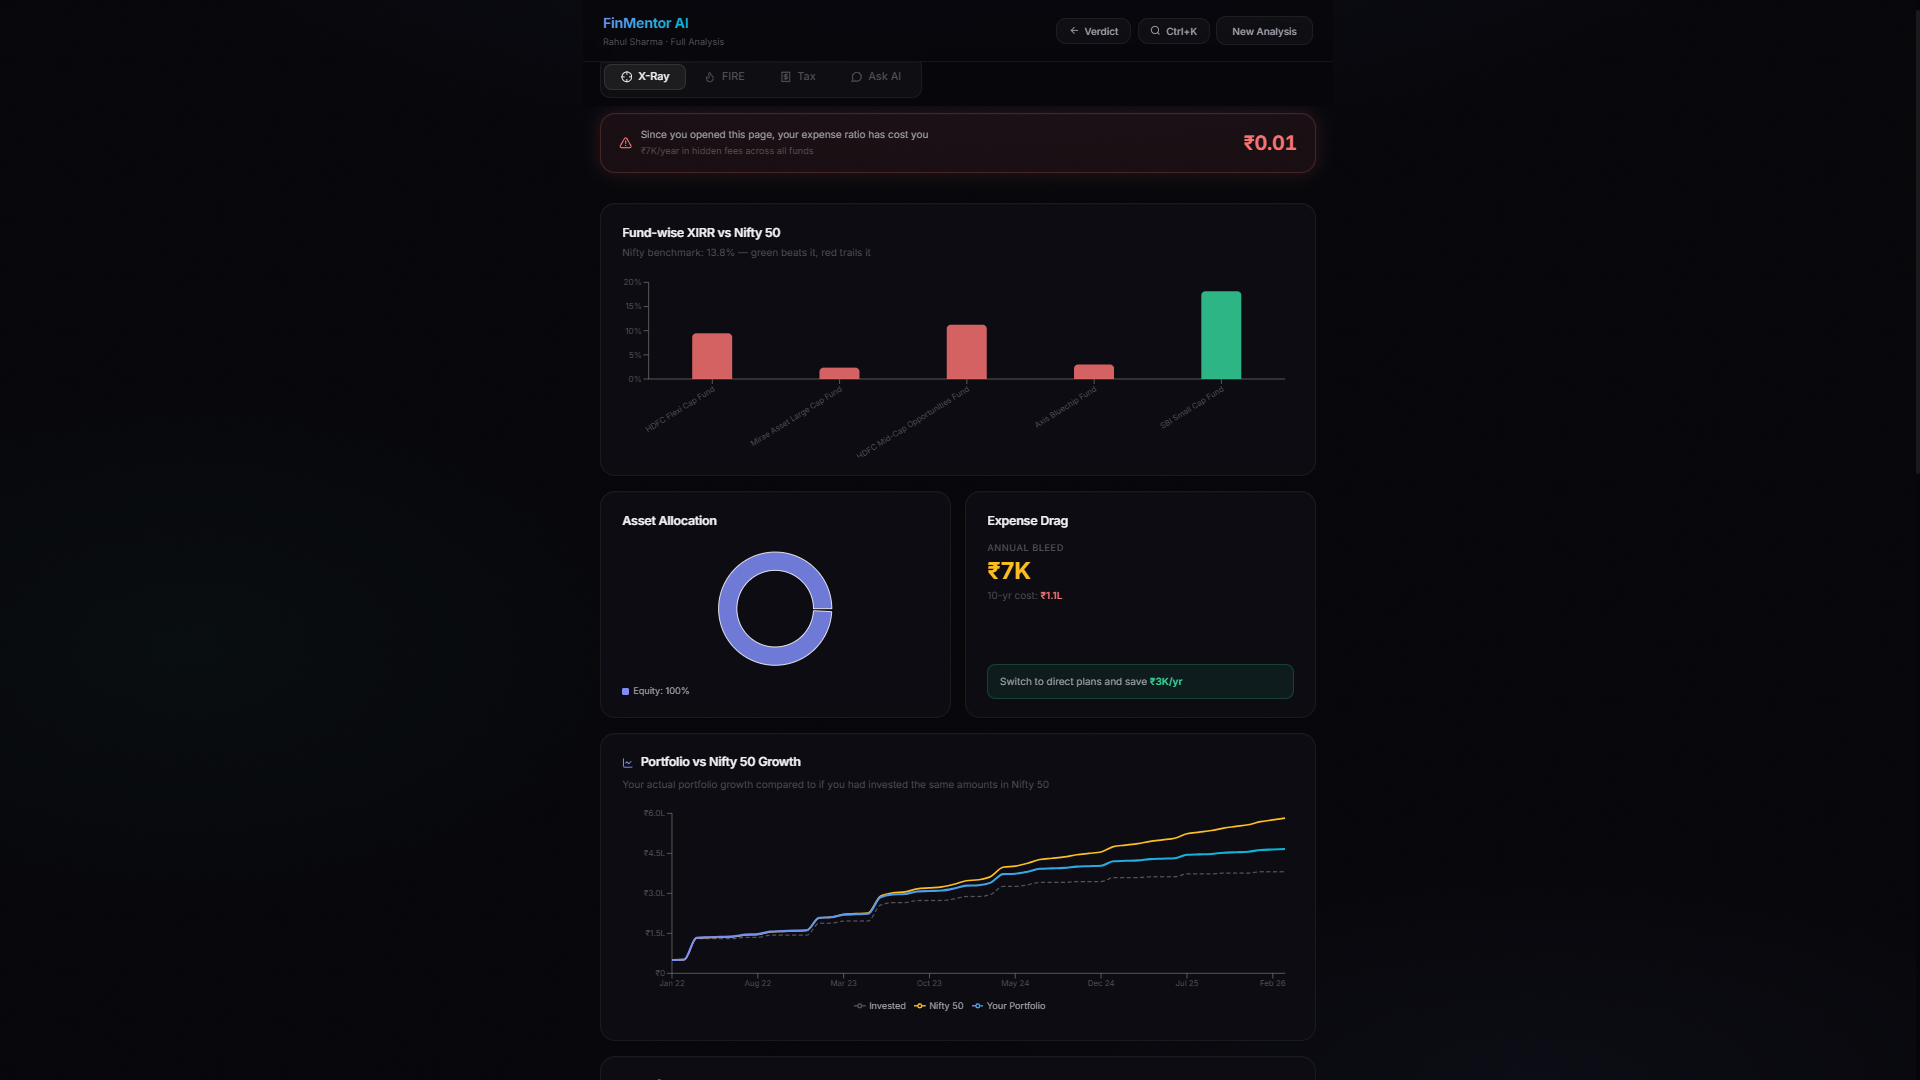
\includegraphics[width=0.23\textwidth]{screenshot_dashboard.png} &
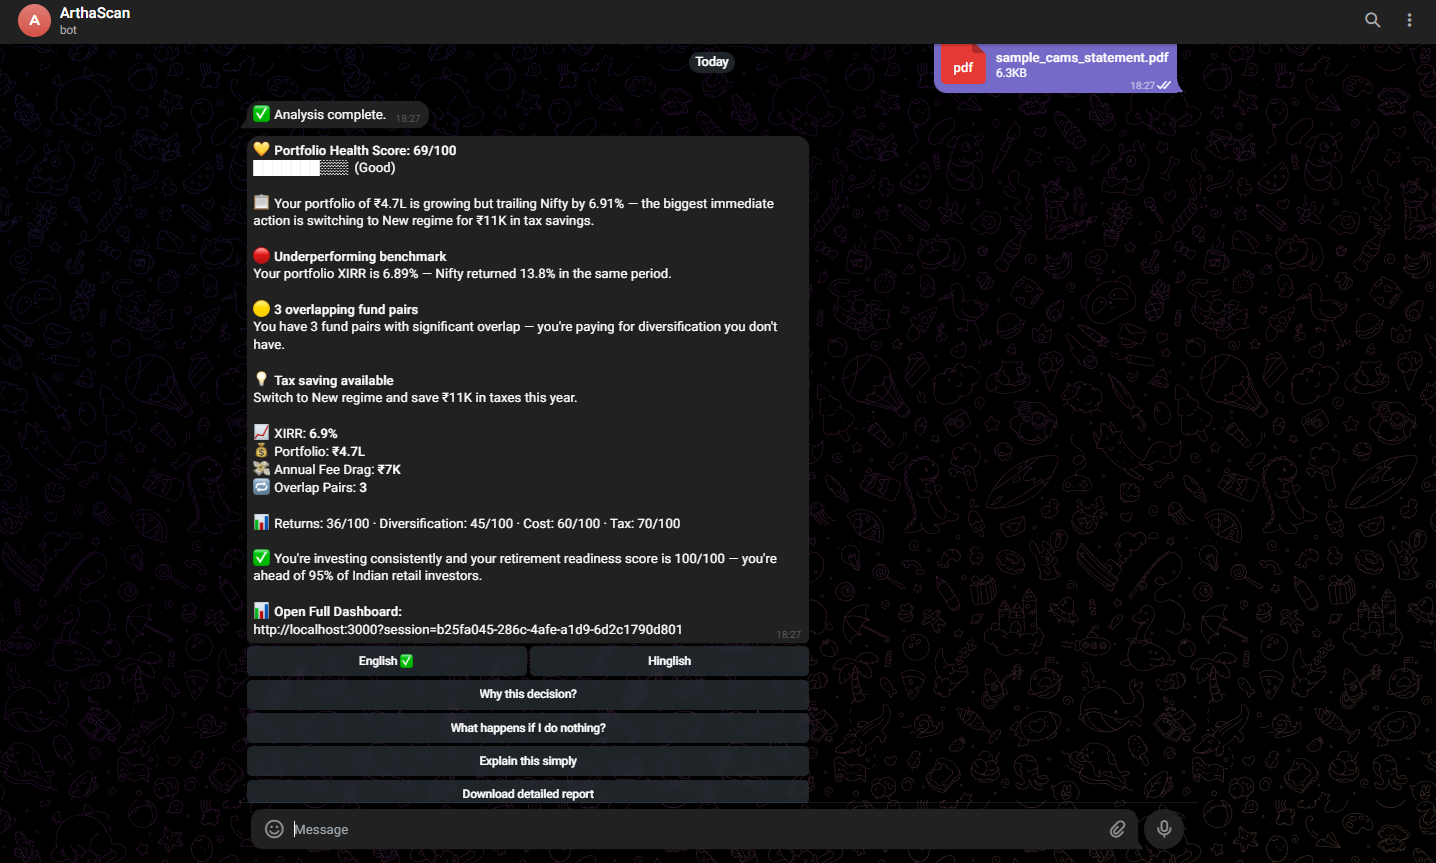
\includegraphics[width=0.23\textwidth]{screenshot_telegram.png} \\[2pt]
{\scriptsize\color{primary}\textbf{Upload \& Extract}} &
{\scriptsize\color{primary}\textbf{Verdict \& Health Score}} &
{\scriptsize\color{primary}\textbf{Dashboard X-Ray}} &
{\scriptsize\color{primary}\textbf{Telegram Bot}} \\
\end{tabular}
\end{figure}

\vspace{-0.5em}
% ─── Extraction ────────────────────────────────────────────────────────────────
\section{I. Multimodal Data Extraction Pipeline}

\small LLMs struggle with dense, tabular CAMS/KFintech statements. Our pipeline uses a multi-strategy approach:

\begin{itemize}[leftmargin=*,nosep]
    \item \textbf{Web Dashboard:} \texttt{pdfplumber} extracts raw text from CAMS PDFs and optional Form~16 documents, then \textbf{Gemini 2.5 Flash} converts it to validated JSON with strict schema prompting.
    \item \textbf{Telegram Bot:} Rasterizes PDFs to 200 DPI PNGs via \texttt{PyMuPDF} for high-accuracy image-to-JSON extraction via Gemini Vision.
    \item \textbf{Self-Healing Loop:} Pydantic validation with recursive re-prompting on malformed output.
    \item \textbf{Regex Fallback:} Silent parser as safety net during API timeouts, ensuring data stability.
\end{itemize}

% ─── Deterministic Engine ──────────────────────────────────────────────────────
\section{II. The Deterministic Financial Engine}

\small In our architecture, the AI is \textbf{``Math-Blind.''} Once data is extracted, it enters a walled-off sandbox where only pure Python algorithms operate. \textbf{No LLM touches a number.}

\begin{multicols}{2}
\small

\subsection{1. XIRR Engine}
Uses \texttt{pyxirr} for exact XNPV/XIRR against historical cashflows --- per-fund and portfolio-wide. 100\% auditable.

\subsection{2. Overlap \& Duplication Detection}
Normalizes stock exposures across funds; pairwise overlap visualized as an interactive \textbf{Network Graph} with severity-coded edges.

\subsection{3. Wealth Bleed Analysis}
Compounds Expense Ratio against Direct Plan baseline over 10~years. Displayed as a \textbf{real-time ticker} counting money lost per second.

\subsection{4. Benchmark Timeline}
Month-by-month portfolio value vs.\ Nifty~50 with identical SIP amounts. \textbf{Dual-line visual proof of alpha.}

\subsection{5. FIRE Retirement Planner}
Goal-based SIP allocation with inflation-adjusted projections. Interactive SIP slider for real-time what-if adjustments.

\subsection{6. Tax Regime Optimizer}
Old vs.\ New regime comparison with deduction gap analysis (80C, 80D, 80CCD, HRA). Computes exact annual savings.

\subsection{7. Portfolio Stress Test}
Loss estimation under Nifty corrections ($-10\%$, $-15\%$, $-25\%$) factoring in equity allocation and beta-adjusted concentration risk.

\end{multicols}

% ══════════════════════════════════════════════════════════════════════════════
\newpage
% ══════════════════════════════════════════════════════════════════════════════

% ─── Health Score ──────────────────────────────────────────────────────────────
\section{III. 6-Dimension Money Health Score}

\small A proprietary scoring framework assessing complete financial wellness beyond simple returns:

\begin{table}[H]
\centering
\small
\setlength{\tabcolsep}{4pt}
\begin{tabularx}{0.95\textwidth}{lll}
\toprule
\textbf{Dimension} & \textbf{Source Engine} & \textbf{Scoring Logic} \\
\midrule
Returns & XIRR Engine & Portfolio XIRR vs Nifty benchmark \\
Diversification & Overlap Engine & Inverse of concentration / overlap penalty \\
Cost Efficiency & Wealth Bleed Engine & Expense ratio vs category average \\
Tax Optimisation & Tax Engine & Regime choice + deduction utilization \\
Emergency Fund & FIRE Engine & Current liquid corpus vs 6-month target \\
Insurance & Tax Engine & Section 80D utilization as insurance proxy \\
\bottomrule
\end{tabularx}
\end{table}
\vspace{-0.5em}

\small Visualized as a \textbf{Radar Chart} with a weighted overall score (0--100), mapped to a \textbf{Peer Percentile Rank} against Indian retail investor benchmarks on an animated gradient bar.

% ─── Presentation Layer ────────────────────────────────────────────────────────
\section{IV. Intelligent Presentation Layer}

\begin{multicols}{2}
\small

\subsection{Voice-Powered AI Chat}
Web Speech API integration with continuous recognition (\texttt{en-IN} locale). Real-time interim transcription, auto-submits on sentence completion. Enables hands-free financial consultation.

\subsection{Action Plan Timeline}
Findings auto-converted into \textbf{prioritized, time-bound steps} (Week~1: Consolidate $\rightarrow$ Week~2: Switch regime $\rightarrow$ Month~1: Increase SIP). Severity-coded with a visual vertical timeline.

\subsection{What-If Life Event Simulator}
Interactive modeling for Bonus, Marriage, New Baby, and Job Switch scenarios. Adjusts projected corpus, readiness score, and gap in real-time with animated transitions.

\subsection{Regulatory Impact Feed}
Recent SEBI, RBI, and Income Tax regulatory changes with \textbf{personalized impact analysis} for the user's specific portfolio and tax situation.

\subsection{Glass-Box Intent Routing}
Math queries bypass the LLM entirely. Explanation Agent translates deterministic facts into English/Hinglish. Guard rails prevent illegal financial advice --- all responses cite underlying calculations.

\subsection{PDF Report Export}
One-click export via CSS print styles (web) and ReportLab-generated PDFs (Telegram). Complete analysis with scores, findings, and action items.

\end{multicols}

% ─── Cross-Channel ─────────────────────────────────────────────────────────────
\section{V. Cross-Channel Architecture}

\begin{tcolorbox}[colback=lightbg,colframe=highlight,boxsep=1pt,left=4pt,right=4pt,top=2pt,bottom=2pt]
\small Both channels converge on a single \textbf{FastAPI backend}. The Telegram bot acts as a thin client, forwarding PDFs to the same \texttt{/analyse} endpoint and formatting the response for Telegram HTML display.
\end{tcolorbox}

\begin{itemize}[leftmargin=*,nosep]
    \item \textbf{Session Persistence:} Analysis results stored as \textbf{file-backed JSON sessions} (survive server restarts).
    \item \textbf{Telegram $\rightarrow$ Web Deep-Link:} One-tap button opens the web dashboard pre-loaded with the same analysis via \texttt{?session=} URL parameter.
    \item \textbf{localStorage Resume:} Web app persists analysis locally for instant resume without re-upload.
    \item \textbf{Multi-Language:} English and Hinglish with one-tap switching on both channels.
\end{itemize}

% ─── Tech Stack ────────────────────────────────────────────────────────────────
\section{VI. Technology Stack}

\begin{table}[H]
\centering
\small
\setlength{\tabcolsep}{4pt}
\begin{tabularx}{0.95\textwidth}{lXX}
\toprule
\textbf{Layer} & \textbf{Web Ecosystem} & \textbf{Telegram Ecosystem} \\
\midrule
LLM & Gemini 2.5 Flash & Gemini 2.5 Flash \\
Backend & FastAPI + Python 3.11 & python-telegram-bot \\
Frontend & React 18 + Recharts + Framer Motion & Telegram Bot API \\
Extraction & pdfplumber + Gemini & PyMuPDF + Gemini Vision \\
Math Engine & pyxirr, NumPy, Pydantic & pyxirr, NumPy, Pydantic \\
Voice & Web Speech API (SpeechRecognition) & --- \\
Persistence & File-backed sessions + localStorage & httpx $\rightarrow$ FastAPI \\
\bottomrule
\end{tabularx}
\end{table}

% ─── Impact ────────────────────────────────────────────────────────────────────
\section{VII. Impact \& Scalability}

\begin{tcolorbox}[colback=action!5!white,colframe=action,boxsep=1pt,left=4pt,right=4pt,top=2pt,bottom=2pt]
\small \textit{If 1,00,000 Indians upload their CAMS statements today, FinMentor AI would surface an estimated \textbf{{\rupee}850 Crore} in hidden expense drag that investors didn't know existed. That's not a feature --- that's a financial awakening.}
\end{tcolorbox}

\vspace{-0.3em}
\begin{multicols}{2}
\begin{itemize}[leftmargin=*,nosep]
    \item \textbf{{\rupee}850 Cr} in hidden fees identified
    \item \textbf{{\rupee}340 Cr} recoverable via Direct plan switches
    \item \textbf{42,000} overlapping fund pairs detected
    \item \textbf{67,000} users with sub-optimal tax regime
\end{itemize}
\end{multicols}

\vspace{0.3em}
\small The architecture is \textbf{model-agnostic}: Gemini can be swapped for Claude, GPT-4, or on-premise models (e.g., LLaVA) without altering the deterministic engines. The math layer never changes regardless of which LLM handles extraction. The file-backed session store can be upgraded to Redis or PostgreSQL for production scale.

\end{document}
